\documentclass{article}
%
% BASIC PACKAGES
\usepackage{amsmath,amssymb,amsthm,enumitem} % Some standard math packages.
\usepackage{titling} % Enables \setlength{\droptitle}
\usepackage{parskip} % Cleaner paragraph display
\usepackage[margin=0.75in]{geometry} % Adjusts margins.
\usepackage[utf8]{inputenc} % Use UTF-8 input encoding instead of default ASCII.
\usepackage{fancyvrb} % Allows Verbatim sections with line numbers and such. Note the capital V.
\usepackage{xcolor} % for text color, e.g. \todo command
\usepackage{ragged2e} % For text alignment environments, e.g. \begin{center}
\usepackage{enumitem} % Allows different list enumerations, like a.) b.) c.)
\usepackage{nameref} % Allows using \nameref{refname} to insert links to sections by title
\usepackage{graphicx} % For \includegraphics

% HYPERLINKS
\usepackage{hyperref} % For \href and \uri
\hypersetup{
  colorlinks=false,
  pdfborder=0 0 0 % No clue what the numbers do, but 0 0 1 is the default, and 0 0 0 disables link boxes.
}

% BIBLIOGRAPHY
\usepackage[english]{babel}
\usepackage[
  backend=biber,
  style=numeric,
  sorting=ynt
]{biblatex}
\addbibresource{bibliography.bib}

% CUSTOM COMMANDS
\newcommand {\todo}[1] {{\textbf{\color{red}#1}}}
\newcommand {\code}[1] {\texttt{#1}}
\newcommand {\term}[1] {\textbf{#1}}

\begin{document}

% Header
\begin{center}
    \Huge Re-implementing a Ruby on Rails Site in Yesod \\
    \large CS 557: Functional Languages @ Portland State University \\
    Dylan Laufenberg, winter 2019
\end{center}

\section{Introduction}

For the last seven years or so, I've been developing and expanding a Ruby on Rails-powered website for a Sacramento, CA soup kitchen named Sharing God's Bounty. I've had mixed feelings about my choice of Ruby on Rails over the last half-dozen years, so this final project provides an excellent opportunity to experiment with a significantly different Web technology stack than any other that I've used. I implement a narrow, vertical slice of functionality to experience and experiment with Haskell across many aspects of server-side code for the Web. I use the Yesod Web framework for my project, and I provide comparisons to my Ruby on Rails experience as appropriate throughout this report. I follow the quick start instructions \cite{yesodQuickstart}, which have provided me with Yesod 1.6.0.3.

Yesod's documentation comes primarily from the Yesod book \cite{ybk}, so a large portion of my work for this project has simply been reading through the book to understand how to utilize this highly sophisticated, mature framework. I don't attempt to introduce or define every concept in Yesod here. Instead, I highlight particularly noteworthy applications of Haskell to the domain of Web application development and discuss how I use Yesod to build out the features I develop for this final project. In particular, I assume the reader knows about Haskell features such as Template Haskell, QuasiQuotes, and language pragmas either through prior knowledge or by reading the Haskell section of the Yesod book \cite{ybkHaskell}.



\part{Learning the Basics}

\section{Resources and type-safe URIs} \label{resourcesAndTSURIs}

One of the first concepts we need to discuss in Yesod, and one of the clearest examples of applying Haskell type safety to an unexpected domain, is the problem of constructing a routing system to bind certain URIs to associated server-side actions.

The most fundamental term here, one which Yesod shares with many other Web frameworks, is the \term{route}, which is a mapping from a URI to server-side code. To represent routes, Yesod uses what it calls resources. A \term{resource} is a \code{data} constructor that acts as the canonical name of the route in views \cite{ybk}. For instance, the default site scaffold includes a static route of the form:

\begin{Verbatim}
/static StaticR Static appStatic
\end{Verbatim}

This line specifies a \code{/static} route, a resource constructor named \code{StaticR} as the name of the route, and a subsite named \code{Static} whose function \code{appStatic} will handle requests on this route \cite{ybkRouting}. In order to create a link to a static file, e.g. an image served as part of a template, we invoke the \code{StaticR} constructor with an appropriate argument. The \code{Static} subsite generates ``static file identifiers`` at compile time \cite{ybkScaffolding}. When we insert a link using a resource constructor:

\begin{Verbatim}
<img ... src="@{StaticR img_logo_png}" ... />
\end{Verbatim}

Yesod generates a correct link to the static resource at compile-time. In this case, the user's browser receives:

\begin{Verbatim}
<img ... src="http://localhost:3000/static/img/logo.png?etag=GVVUzjtL" ... />
\end{Verbatim}

\subsection{Benefits of Resources}

There are two primary benefits to this approach, both of which leverage Haskell features from class (albeit at a very advanced level).

\paragraph{Check links at compile time} Yesod uses resources to generate correct links at compile-time, which allows it to check whether said links are valid and raise compile-time errors if any problems are detected. In this case, the Static subisite checks the identifier \code{img\_logo\_png} against all generated static file identifiers. If it finds a match, it inserts the correct link. If not, then GHC raises an error. For instance, if we mistakenly specify a JPG logo:

\begin{Verbatim}
<img ... src="@{StaticR img_logo_jpg}" ... />
\end{Verbatim}

GHC detects the issue for us and (rather obtusely) notifies us of the issue with a compile-time error:

\begin{Verbatim}
    • Variable not in scope: img_logo_jpg :: Route Static
    • Perhaps you meant ‘img_logo_png’ (imported from Import.NoFoundation)
    |
163 |             $(widgetFile "default-layout")
    |               ^^^^^^^^^^^^^^^^^^^^^^^^^^^
\end{Verbatim}

In effect, Yesod automatically tests every internal link at compile time, without the need to manually write tests against the generated HTML. We, the developers, need to test our functions for generating links, then Yesod takes care of the rest for us. In this case, I feel comfortable as a developer taking it on faith that the static file subsite is well-tested.

\paragraph{Refactor routes with confidence} Generating links at compile time also eliminates an entire class of common and nefarious errors: broken links. Updating or moving routes is a common occurrence in Web application development, even with careful planning. Yesod makes this safe and automatic by generating all such links from resource constructors at compile time. To change the route across the entire application, all we need to do is change the route definition:

\begin{Verbatim}
/dynamic StaticR Static appStatic
\end{Verbatim}

And all of our generated links to that route automatically update when we recompile:

\begin{Verbatim}
<img ... src="http://localhost:3000/dynamic/img/logo.png?etag=GVVUzjtL" ... />
\end{Verbatim}

% This is also a great point of comparison to Ruby or Python, where this is impossible by the very nature of the languages.



\section{Shakespearean Templates}

Yesod provides domain-specific languages (DSLs) over HTML, CSS, and Javascript, all named after Shakespearean characters. In converting my site, I migrated the HTML, CSS, and Javascript, in that order. (For the full, reference versions of all information in this section that's not otherwise cited, see \cite{ybkShakes}.)

All of Yesod's DSLs provide a common set of interpolation features:

\begin{itemize}
  \item \term{Variable interpolation} All variables in scope when a template is rendered are available through variable interpolation. For instance, in my main site template, I write

    \code{<title>\#\{pageTitle pc\} - Sharing God's Bounty}

    to insert the value of \code{pageTitle pc} as part of the HTML title.

  \item \term{Resource interpolation} We can insert type-safe URIs via \code{@\{routeR\}} resource interpolation, as discussed in \nameref{resourcesAndTSURIs}.

  \item \term{Template interpolation} We can embed templates in other templates by writing \code{\^{}\{templateName\}}. This is safe in that it only allows embedding of templates of the same type and, of course, provides all the usual compile-time guarantees for both templates. \todo{Add reference to Mixins section?}
\end{itemize}

\subsection{Hamlet}

Yesod uses Hamlet as its HTML DSL. Hamlet is similar to HTML, with a few distinguishing features.

\paragraph{Significant whitespace} Hamlet templates infer closing tags from indentation levels. When you write, for instance, \code{<div>}, everything that should appear inside this tag must be nested below it. A matching closing tag is automatically inserted at the correct place in the generated HTML. 

\paragraph{Class and ID shorthand} Hamlet templates provide shorthand for specifying classes and IDs by prefacing a class or ID name with a \code{.} or a \code{\#}, respectively. This shorthand even works with multiple classes, by writing either \code{<div .foo .bar>} or \code{<div ."foo bar">}. Either form generates the final HTML \code{<div class="foo bar"></div>}. To be honest, I tried these forms with the intention of exposing a shortcoming of Hamlet, and I was shocked to see that it handled both cases beautifully!

\paragraph{Example} To see these features in action, let's take a look at my mobile navigation menu. The Hamlet representation is as follows: \todo{UPDATE THIS EXAMPLE with the ``final'' version! It'll be WAY more impressive!}

\begin{Verbatim}
<nav .mobile>
  <ul>
    <li>Menu items go here. 
  <h2>
    Menu
\end{Verbatim}

Which compiles to:

\begin{Verbatim}
<nav class="mobile"><ul><li>Menu items go here. </li>
</ul>
<h2>Menu</h2>
</nav>
\end{Verbatim}

\paragraph{Shortcomings} There are, unfortunately, a number of shortcomings to Hamlet. First and perhaps most importantly, none of the four templating DSLs provide the strong, compile-time guarantees of correctness that we expect in Haskell, even though Hamlet in particular feels like it could. As a new user, I was genuinely surprised to learn that Hamlet doesn't raise compile-time errors for invalid tags! For instance, when I mistakenly wrote \code{<image ...>}, Hamlet happily generated both opening and closing \code{image} tags, which, understandably, confused both Firefox and me.

Second, although Hamlet knows that some tags like \code{img} are self-closing, it doesn't insert the closing \code{/} at the ends of such tags.

Third, Hamlet \emph{does not} check whether classes and IDs written in Hamlet notation exist in linked Cassius or Lucius files!

Fourth, the HTML produced seems to be both arbitrary and virtually unreadable in its structure. The navigation example above is Hamlet's output, verbatim, and this is with minimization disabled! What particularly irks me about this oversight is that Hamlet \emph{outright requires} proper indentation and spacing! Why it doesn't simply carry this indentation through to the final HTML is beyond my comprehension.

\subsection{Lucius}
To represent CSS, Yesod uses two, equivalent DSLs: Lucius, which is ``a superset of CSS'' \cite{...}, and Cassius, which uses significant whitespace instead of curly braces. I chose to use Lucius to ease the process the migration from Ruby on Rails.

Lucius and Cassius both present broadly similar feature sets to Sass, which my Ruby on Rails app uses for its CSS. In fact, in searching for help on Lucius mixins, I found a question by a Sass user who was similarly struggling with the Lucius equivalent \cite{...}. (More on that in the \todo{CORRECT Mixins} section.) Put simply, Lucius and Cassius aim to ease the process of writing CSS, \emph{not} to provide strong compile-time guarantees of the correctness of CSS.

\subsection{Basic features}

Lucius supports fairly standard features to simplify generating CSS. In addition to interpolation, it supports another, immensely useful feature: nesting selectors to reduce repetition. Other than the surprising (and unfriendly) syntactic detail that we write \code{@foo} to define a variable and \code{\#\{foo\}} to use it, Lucius feels familiar after working with Hamlet. With this understanding, I began migrating my Sass by writing some Lucius variables at the top of my \code{.lucius} file:

\begin{Verbatim}
@textcolor: #333;
@pageBGDark: #382916; /* Brown */
@pageTextLight: white;
@spacing: 20px;
@halfSpacing: 10px;
\end{Verbatim}

Here, \code{@spacing} and \code{@halfspacing} supported the grid on which I originally designed the layout and opened up a new possibility that, should I ever wish to adjust this grid, I might well be able to do so simply by changing these variables. However, this potential is limited somewhat by encountered another, unfortunate limitation I found while experimenting with this new idea: Lucius variables cannot invoke other Lucius variables. When we write, for instance: 

\begin{Verbatim}
@spacing: 20px;
@halfSpacing: calc(#{spacing}/2);

body {
  margin: 0 #{halfSpacing};
}
\end{Verbatim}

Lucius generates the CSS:

\begin{Verbatim}
body {
  margin: 0 calc(#{spacing}/2);
}
\end{Verbatim}

If Lucius supported either nested variables or some notion of compile-time calculation with variables, I might be able to scale nearly every element on the page according to the \code{@spacing}. It's disappointing that Yesod ships with this limitation, but it downright disheartens me that Lucius does not even notice that it's parsing very clearly invalid CSS!

Then, I updated my CSS to take advantage of all three forms of interpolation as well as nested selectors.

Topics:
\begin{itemize}
  \item Hamlet: went pretty smoothly, Initially had to cut out lots of features as NYI.
  \item Lucius/Cassius: oh, man. Whole subsection(s), whole big thing.
\end{itemize}

%   Migrate main HTML template, creating a list of features snipped out:
%     Christmas mode
%     Mobile menu
%     Meals served & last meal
%     Announcements
%     Main menu
%     Flash notice and alert
%     Footer: current year
%     Footer: login link
%   Migrate main CSS stylesheet to Lucius:
%     Integrate variables where appropriate
%     Convert image URLs to StaticR resources for compile-time safety
%     Nest CSS with shared tags (e.g. all .masthead selectors)
%     Mixins:
%       - Can't use the Yesod book's quasi-quoters readily in the scaffolded Yesod site, either in the Lucius file or in src/Foundation.hs (where defaultLayout is defined), because I need to annotate a type manually to deal with string overloading (Text vs. [char]), and I can't easily find the type of the QuasiQuoter used (because it far exceeds my level of knowledge of Haskell, GHCI, QuasiQuoters, and Yesod). 
%       - Google doesn't have any usable documentation on this that I've found.
%       - The Yesod wiki seems to be broken
%       - The LTS build of Yesod appears to be over 5 years old and appears to predate this: https://www.yesodweb.com/blog/2013/07/runtime-lucius-mixins
%       - Because of either Stack or Yesod's package management, I can't import Text.Lucius from GHCI to check the type.
%       - However, I eventually realized that I could trick Stack/Yesod into telling me the correct type simply by writing a dummy type and checking the 'Expected' output! Oputput:
%               • Couldn't match expected type ‘Mixin’ with actual type ‘Int’
%               • In the first argument of ‘Text.Internal.Css.CDMixin’, namely
%                   ‘(centering "200px")’
%                 In the expression: Text.Internal.Css.CDMixin (centering "200px")
%                 In the expression:
%                   ((Text.Shakespeare.Base.DerefBranch
%                       (Text.Shakespeare.Base.DerefIdent
%                          (Text.Shakespeare.Base.Ident "centering")))
%                      (Text.Shakespeare.Base.DerefString "200px"), 
%                    Text.Internal.Css.CDMixin (centering "200px"))
%               |
%           163 |             $(widgetFile "default-layout")
%               |               ^^^^^^^^^^^^^^^^^^^^^^^^^^^
% 
%           --  While building package final-project-0.0.0 using:
%                 /home/dylan/.stack/setup-exe-cache/x86_64-linux-tinfo6/Cabal-simple_mPHDZzAJ_2.2.0.1_ghc-8.4.4 --builddir=.stack-work/dist/x86_64-linux-tinfo6/Cabal-2.2.0.1 build lib:final-project --ghc-options " -ddump-hi -ddump-to-file"
%               Process exited with code: ExitFailure 1
%       - I changed the type annotation to Text -> Mixin and it worked perfectly.
%       - I learned while creating the HTML template that older versions of Yesod won't recognize new static files unless I stack clean && stack exec -- yesod devel, and that the LTS release I received from Stack is old enough that it has this issue.
%       - I learned while trying to get Mixins working that I also have to clean and rebuild if I change a Lucius mixin.
%     Limitation of variables:
%       - I tried converting my 20/10-pixel spacing to @spacing and @halfSpacing, with @halfSpacing defined as @halfSpacing = calc(#{spacing}/2);, but it doesn't process #{spacing} or even produce a compile error! It actually produces incorrect CSS!
%       - I found that if I leave a semicolon off a variable, it will also produce invalid CSS! What gives?!
%     Next steps:
%       1. Get good dummy content in
%       2. Get the CSS working well and looking right!
%       3. Continue refactoring the CSS


\section{Skipped sections}

In order to maximize the value of this Yesod experiment, I skip over a number of topics that the Yesod book covers in detail. I don't touch them in my implementation except where absolutely necessary, though I may refer to them as needed. Because I'm not directly and explicitly working with them, I won't discuss them directly here. See the Yesod book (as needed) for background information on:

\begin{itemize}
  \item Widgets
  \item The Yesod typeclass
  \item Forms
  \item Sessions
\end{itemize}

\part{Adding New Features}

\section{Storing pages in a database}

Now that we've covered most of the basics, we can look at adding new features to the scaffolded application. Given the stated scope and the time constraint of the project, our focus is on adding a narrow, vertical slice of features designed to let us learn about, experience, and discuss Haskell and Yesod. These features are \emph{not} designed to be production-ready but rather to fulfill these stated objectives. The first set of new features we add includes the ability to store pages in a database, associate them with URIs, and display them.

\subsection{Adding a table to the database}

Our first order of business is to learn enough about Persistent, Yesod's database abstraction layer \cite{ybkPersistent}, to create a new table. Persistent leverages Haskell data types to provide myriad type-safety guarantees going both to and from a backing store (in our case, SQLite). Persistent defines a sum type, \code{PersistValue}, whose constructors map to supported value types we can store in the database. The Yesod book defines \code{PersistValue} as follows \cite{ybkPersistent}:

\begin{Verbatim}[samepage=true]
data PersistValue
    = PersistText Text
    | PersistByteString ByteString
    | PersistInt64 Int64
    | PersistDouble Double
    | PersistRational Rational
    | PersistBool Bool
    | PersistDay Day
    | PersistTimeOfDay TimeOfDay
    | PersistUTCTime UTCTime
    | PersistNull
    | PersistList [PersistValue]
    | PersistMap [(Text, PersistValue)]
    | PersistObjectId ByteString
    -- ^ Intended especially for MongoDB backend
    | PersistDbSpecific ByteString
    -- ^ Using 'PersistDbSpecific' allows you to use types
    -- specific to a particular backend
\end{Verbatim}

Meanwhile, columns are represented by the \code{PersistField} typeclass and tables are represented by the \code{PersistEntity} typeclass \cite{ybkPersistent}.

\paragraph{The models file} The scaffolded Yesod site reads its Persistent configuration from the file \code{config/models}, which defines the database configuration using a Persistent DSL \cite{ybkScaffolding}. The DSL features we utilize are as follows:

\begin{itemize}
  \item \term{Tables} are represented as top-level headers with no indentation. They should be CamelCased with initial capital.
  \item \term{Columns} are represented as lines indented under the table to which they belong. Three, space-separated fields make up a column declaration: 
  \begin{enumerate}
    \item The column name (camelCased with initial lowercase, for use as the name of a \code{PersistField}).
    \item The column type, as a \code{PersistValue} constructor type.
    \item Optionally, any additional attributes, such as \code{Maybe} to allow the column to be null.
  \end{enumerate}
  \item \term{Unique constraints} are represented at the same indentation level as columns, as follows:
  \begin{enumerate}
    \item The unique constraint name (CamelCased with initial capital).
    \item The names of any columns to be included in the constraint, space-separated.
    \item Optionally, the \code{force!} directive to allow a unique constraint involving a nullable column. (This is not allowed by default because Haskell and SQL differ in their definitions of equality of null values \cite{ybkPersistent}.)
  \end{enumerate}
\end{itemize}

\paragraph{Defining a new table}

For the purposes of this project, we simply need one table that provides enough information to represent pages and, eventually, a single, unified navigation menu. Following the example of the real Sharing God's Bounty website, we represent a page as a title, a path (i.e. the relative path from the root of the site to the page), and some contents to be displayed in an article body. Meanwhile, to support menus, each page must be representable in the menu, which requires a numeric sorting order (so we can reorder pages) and some display text. The path and both menu-related fields should be nullable so that we can de-list a page completely if desired, making it entirely inaccessible to the public.

We complete our design with two unique constraints. First, no two pages should be allowed to have the same path, though this might be perfectly plausible under a different site architecture. Seecond, no two pages should be allowed to have the same numeric menu order.

These design specifications allow us to produce a full model in the Persistent DSL:

\begin{Verbatim}[samepage=true]
BasicPage
    title Text                        -- The title of the page
    path Text Maybe                   -- The path to the page (nullable)
    menuOrder Int64 Maybe             -- The numeric order of the page in the menu (nullable)
    menuText Text Maybe               -- The text of the page's menu entry (nullable)
    content Text                      -- The page's body content
    UniquePath path !force            -- The path must be unique but may still be null
    UniqueMenuOrder menuOrder !force  -- The menu order must be unique but may still be null
\end{Verbatim}

\paragraph{Migrating the schema} For the uninitiated, database migrations are a standard notion of capturing changes to the database schema in a programmatic and reproducible way. In Ruby on Rails, we write migrations manually (or use a command-line utility to generate both our skeletal models and skeletal migrations). Yesod goes at least one step further: it automatically generates and runs migrations, when it's safe to do so, by comparing the Persistent schema to the database schema \cite{ybkPersistent}. Potentially destructive migrations must be written by hand. (We avoid them to narrow the scope of this project.) Thus, all that's required to create our table and teach Yesod how to handle it safely is to create the above specification in the Persistent DSL!

\paragraph{Reflections} Persistent is a bit of an odd duck. Then again, so is Ruby on Rails' ActiveRecord. I have taken issue with a number of Yesod's choices and limitations. Given that, I feel I need to highlight that my experience with Persistent has been stellar! This is the most remarkably helpful database DSL I have personally seen to date. It's cryptic at first, which is unsurprising in Yesod, but I am truly awe-struck by Persistent's expressive power!

Having said that, I take the same issue with Persistent that I take with ActiveRecord. Both DSLs attempt to solve the database problem space entirely in their host languages. In doing so, both DSLs take reductive views of databases that belie the power of a full-fledged DBMS. Both DSLs are well-suited to simple data stores like SQLite. As a SQL-literate developer, though, I prefer to take full advantage of a highly tuned, enormously powerful DBMS like Postgresql or Microsoft SQL Server. It is my personal opinion that when using a fully featured DBMS to its full advantage, a heavy-handed database abstraction layer simply gets in the way. Perhaps Persistent might work well in this use case with its migrations disabled (and without utilizing unique constraints), but I have my doubts. In either case, this particular query is well beyond the scope of this project.



\section{Adding a dynamic route}

In order to create a new route to receive requests for these database-backed pages, we first need to learn a bit more about Yesod's routing system. First, we'll discuss more advanced routes, and then we'll discuss the handlers that process them.

\subsubsection{Routing with PathPieces}

Yesod breaks routes into pieces, delimited by \code{/}, and parses them using data types that are instances of either the \code{PathPiece} or \code{PathMultiPiece} tyepclasses. It does so in a way that protects us from the details of parsing full routes and provides us with one, canonical URI for any given page \cite{ybkRouting}. There are three types of path pieces:

\begin{itemize}
  \item \term{Static text} must be matched exactly. The \code{/static} route discussed previously is static text.
  \item \term{Single pieces} are a single token (as defined by the \code{/} delimiters in the URI). We denote a single piece with the \code{\#} symbol followed by the name of a type that's an instance of the \code{PathPiece} type class.
  \item \term{Multi-pieces} can match any number of pieces. We denote multi-pieces with the \code{*} symbol followed by an instance of the \code{PathMultiPiece} typeclass. A multi-piece must be the last piece in a route.
\end{itemize}

\paragraph{Conversions} The \code{PathPiece} and \code{PathMultiPiece} typeclasses require us to define two-way conversions. \code{PathPiece} requires conversions between \code{Text} and the instance type. \code{PathMultiPiece} requires conversions beetween \code{[Text]} and the instance type. Converting from \code{Text} or \code{[Text]} returns a \code{Maybe} value, which allows us to guard against invalid input and guarantee that we're passing valid inputs into our route handlers. For instance, a multi-piece may enforce arbitrary constraints in its function \code{\frenchspacing fromPathMultiPiece :: PathMultiPiece s => [Text] -> Maybe s}; if it returns \code{Nothing}, the handler is never even invoked.

\paragraph{Ambiguous routes} By default, Yesod disallows routes that overlap and thus provide ambiguity. We can (and, in our case, must) override this behavior and explicitly allow certain routes to overlap by prefacing them with a \code{!} symbol. Yesod's rule when multiple routes match, which is common in routing systems, is that the first route wins \cite{ybkRouting}.

\subsubsection{Adding the route}

Our route itself is conceptually very simple: it will attempt to match any page that has not already matched a route against the known paths in our new database table. We'll use a multi-piece to allow pages to nest as needed, and we'll name our resource after the \code{BasicPath} table. Since only the \code{GET} HTTP method makes sense here, we will restrict our route to that method:

\begin{Verbatim}
!/*PagePath BasicPageR GET
\end{Verbatim}

The Yesod book does not precisely describe where to place our definition for \code{PagePath}'s membership in the \code{PathPiece} typeclass, but perhaps GHC can help us out. By running the application with the route (but without a handler or a definition for \code{instance PagePath PathPiece}), we can see where the definition is needed and make an educated guess about where it might belong. Sure enough, we see a helpful error (edited for clarity):

\begin{Verbatim}
[ 6 of 12] Compiling Foundation       ( src/Foundation.hs, ...)

src/Foundation.hs:68:1: error:
    Not in scope: type constructor or class ‘PagePath’
   |
68 | mkYesodData "App" $(parseRoutesFile "config/routes")
   | ^^^^^^^^^^^^^^^^^^^^^^^^^^^^^^^^^^^^^^^^^^^^^^^^^^^^

\end{Verbatim}

Following the Yesod book's example \cite{ybkRouting}, we define our own \code{PagePath} type and define its instantiation into \code{PathMultiPiece} (as well as a few base classes), and we place the definition at the bottom of \code{src/Foundation.hs}:

\begin{Verbatim}
-- Define the PagePath type needed for our BasicPageR route.
newtype PagePath = PagePath Text
  deriving (Eq, Show, Read)

-- Define converstions between PathPath and Text.
instance PathMultiPiece PagePath where
  -- toPathMultiPiece converts from a PagePath to [Text].
  -- The essential task here is to break a relative path such as
  --   "/foo/bar/baz"
  -- or
  --   "/foo/bar/baz/"
  -- to a list of tokens. In either case above, correct
  -- tokenization would be:
  --  ["foo", "bar", "baz"]
  --
  -- To do this, we'll unpack our Text to a String
  -- for pattern-matching, then use Data.Text.splitOn 
  -- to split our Text on '/' characters while safely
  -- ignoring a leading '/'. We'll take special care
  -- to handle the case of p="/", since T.splitOn
  -- will incorrectly yield ["", ""].
  toPathMultiPiece (PagePath p) = 
    case T.unpack p of
      [] -> []
      "/" -> []
      ('/':rest) -> T.splitOn "/" (T.pack rest)
      _ -> T.splitOn "/" p
        

  -- fromPathPiece converts from [Text] to a PagePath.
  -- We could query the database here to verify that
  -- the path exists, but that functionality is best
  -- left to the handler, for a variety of reasons.
  -- We simply need to join a list of Text objects
  -- with '/' characters, plus a leading '/' character.
  -- In the case of [], we want to produce the value "/"
  -- so that "/" can represent the homepage path in our
  -- DB, following the existing scheme.
  fromPathMultiPiece ts =
    case ts of
      [] -> Just (PagePath "/")
      _  -> Just (PagePath (concat $ map ("/" ++) ts))
\end{Verbatim}

\emph{Note: I assume there's a better way to handle overloaded strings than to unpack, pattern-match, and re-pack, but I had to learn about working with Text values on-the-fly, and I'm way over 32 hours on this project as-is. In terms of performance impact, this website gets 30 requests a day on an exceptionally busy day near Christmastime, so worrying about efficiency here would be a highly premature optimization.}

To verify that our links work correctly, we provide a temporary, initial handler that simply displays the parsed \code{PagePath} in the body of our templated page:

\begin{Verbatim}
getBasicPageR :: PagePath -> Handler Html
getBasicPageR (PagePath path) = defaultLayout $ do
      case path of
        "/" -> [whamlet|Home page: /|]
        _ -> [whamlet|Path: #{path}|]
\end{Verbatim}

Sure enough, visiting \code{localhost:3000} produces a beautiful Bounty webpage with the body text:

\begin{Verbatim}
Home page: /
\end{Verbatim}

And visiting \code{http://localhost:3000/abc/def} produces the body text:

\begin{Verbatim}
Path: /abc/def
\end{Verbatim}

Now we can add database interactivity as part of a real handler.

\subsection{Adding the handler}

Our route handler, in \code{src/Handler/BasicPage.hs}, is as follows:

\begin{Verbatim}
{-# LANGUAGE TemplateHaskell #-}
{-# LANGUAGE OverloadedStrings #-}
{-# LANGUAGE QuasiQuotes #-}

module Handler.BasicPage where

import Import

getBasicPageR :: PagePath -> Handler Html
getBasicPageR (PagePath pagePath) = do
      -- Try to retrieve the page from the database by looking up
      -- the path we received from the BasicPageR route.
      maybePage <- runDB $ getBy (UniquePath (Just pagePath))
      case maybePage of
        -- We received a valid page! Great!
        -- We'll unpack just what we need, discarding the rest,
        -- and render the layout by following the same basic steps
        -- as the default HomePageR handler.
        Just (Entity _ (BasicPage title _ _ _ content)) 
          -> defaultLayout $ do
                setTitle (toHtml title)
                $(widgetFile "basicpage")
        Nothing -> notFound -- No page with this path exists in the DB.
\end{Verbatim}

Let's talk about each part in a bit more detail.

First, we use the \code{getBy} function from Persistent to retrieve a page by its path. The \code{getBy} function accepts a unique constraint as its sole argument. From this argument, it infers the needed data types, the table to check, and the column(s) to check. (Ah, the power of the Haskell type system!) In loose terms, it takes variadic arguments: it accepts a unique constraint value, but that value's constructor may require arbitrary arguments. We wrap it in \code{runDB}, which is a convenience function the Yesod scaffolded site provides to pull from a pool of database connections.

Next, we unpack the \code{Maybe (Entity BasicPageId BasicPage)} value we received. If it's \code{Nothing}, the database had no matching row, so we simply use the \code{notFound} helper to terminate our handler with an appropriate response. If we did receive a matching row, then we unpack the fields we need (namely \code {title} and \code{content}), create a widget with those names in scope, and pass the widget into the \code{defaultLayout} renderer.

A \term{widget} is a key concept we skipped previously, but in very brief form, it's comprised of snippets of Hamlet, Lucius, Cassius, and/or Julius code, packed together in a format that Yesod is able to handle intelligently as a single unit. In our case, we just need an exceptionally simple \code{templates/basicpage.hamlet} file:

\begin{Verbatim}
<h1>#{title}
#{content}
\end{Verbatim}

This renders the body of any given page as a widget, using the values we unpacked from the database. When in the default template we invoke:

\begin{Verbatim}
^{widget}
\end{Verbatim}

Yesod renders this widget for us.

\emph{Note: I gloss over some minor details here, but to follow along, you'll need to add the new handler to the Cabal file and src/Foundation.hs, probably comment out your HomeR route (and lines that GHC warns you are unused once you remove that route), and tweak your scaffolded authentication. GHC will guide you, for the most part, as it guided me.}




\section{Adding menus}

Our \code{BasicPage} database table and its associated Haskell type have the three key fields we need in order to represent a site navigation menu: paths, titles, and numeric orders for all pages. All three are optional so that we can remove pages from the Web as needed. (We use this on the live Bounty site for Christmas event pages, for instance.) Having gained experience writing Persistent code, handlers, and Hamlet, we now turn our attention to one, final feature for this project: adding the site navigation menu.

Given the work already done, adding a menu is actually remarkably simple (although getting the code exactly right is challenging the first time, since the Yesod book assumes a lot of unstated but important details about, e.g., where to place certain code or what TemplateHaskell is generated for various data types). We place our code in the \code{defaultLayout} function definition in \code{src/Foundation.hs}, since the menu must be defined for any page that uses this layout (otherwise the template will not compile). The first step is to retrieve a list of menu items from the database (sorted by menu order) and unpack it from the monad that \code{runDB} returns:

\begin{Verbatim}
pageList <- runDB (selectList [] [Asc BasicPageMenuOrder])
\end{Verbatim}

Next, we need to process the results in a few ways. First, we only want pages where the path, menu text, and menu order are all non-null. Second, we only actually need the path and menu text of each page. A somewhat advanced list comprehension can take care of this for us:

\begin{Verbatim}
let menuItems = 
      [(pagePath, title) 
        | (Entity _ 
                 (BasicPage _ 
                            (Just pagePath) 
                            order
                            (Just title) 
                            _)) <- pageList,
          order /= Nothing]
\end{Verbatim}

by using \code{(Just pagePath)} and \code{(Just title)}, we automatically filter out any \code{Nothing} values for these fields and unpack the values from these \code{Maybe} types at the same time. We take a different approach for \code{order} because we don't need to store this value and we don't want GHC to warn us that it's an unused value; instead, we simply retrieve it, guard against \code{Nothing} values, and throw it away.

Finally, in \code{templates/default-template.hamlet}, we need to add identical code to both our mobile navigation and main navigation menus. (If time allowed, we would create a new widget, but for the sake of the project, we simply insert the code directly into the template.) We replace our stubbed menus (see section \nameref{hamlet}) with Template Haskell code:

\begin{Verbatim}
<nav .mobile>
  <ul>
    $forall (path, title) <- menuItems
      $with curpath <- BasicPageR (PagePath path)
        $if Just curpath == mcurrentRoute
          <li .current>
            <a href=@{curpath}>#{title}
        $else 
          <li>
            <a href=@{curpath}>#{title}
\end{Verbatim}

This bit of code iterates over \code{menuItems}, extracting \code{path} and \code{title} from each tuple. For each unpacked tuple, it creates a \code{BasicPageR} resource we can use to generate type-safe links. It inserts a list item and a link for each menu item, applying the \code{current} class to the list item if and only if the item's path is the current page.



\section{Verifying our new features}

To verify that all of the above work as intended, we create a database instance that tests each of these cases, and we verify that the generated web page is correct. Using DB Browser for SQLite \cite{sqliteBrowser}, we populate our data as shown in Figure \ref{fig:db}. Then, by visiting the TestNest page, we can verify a number of items visually in this screenshot of our project's final result, as shown in Figure \ref{fig:site}. Observe that:

\begin{enumerate}
  \item The template displays correctly.
  \item The template inserts the \code{basicpage} widget correctly.
  \item The dynamic route handles complex, nested URIs correctly.
  \item The menu code processes the database instance correctly, including edge cases, i.e. pages where the path, menu title, or menu order is null are not shown in the site's menu.
\end{enumerate}

\begin{figure}[h]
  \centering
  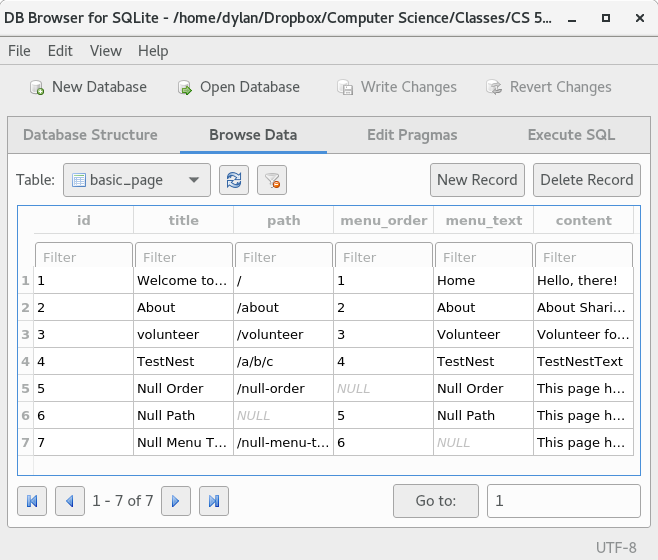
\includegraphics[width=4.4in]{db.png}
  \caption{Our database test instance.}
  \label{fig:db}
\end{figure}

\begin{figure}[h]
  \centering
  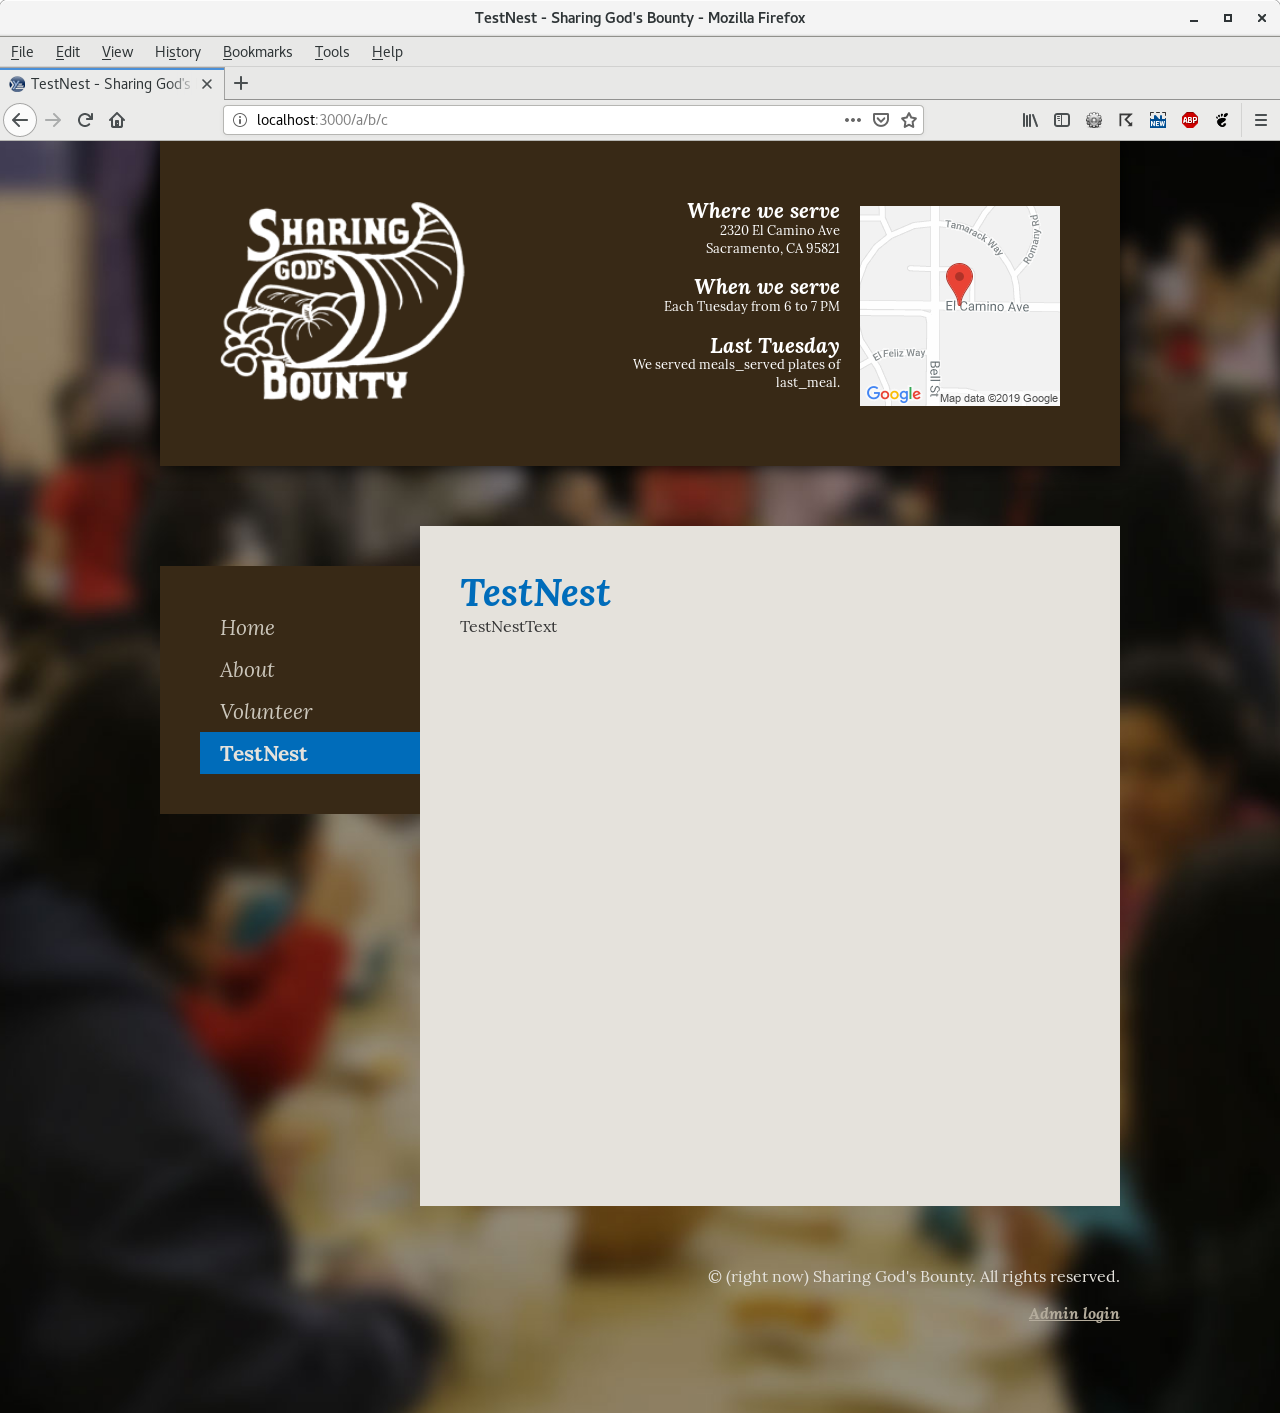
\includegraphics[width=\linewidth]{site.png}
  \caption{Our final website.}
  \label{fig:site}
\end{figure}

\emph{Note: I've tested these features a great deal by clicking through the various pages and hand-checking each attribute as I change it. I sum up all of these checks in this one, informative screenshot to save time, space, and ink.}

\clearpage


\section{Final reflections}

For me, one of the biggest questions all term has been, ``How practical is Haskell in the real world?'' Although we had a guest speaker who uses Haskell in his professional work, I have found my own experience of redoing a real, in-the-wild project from another language to be particularly illuminating. In some ways, Yesod and thus Haskell shines --- Persistent's DSL and auto-migrations are gleaming examples of Haskell's excellence! In other ways, Yesod and thus Haskell suffers by comparison --- Persistent, for instance, entirely lacks Ruby on Rails' persistence abstractions that make working with live data nearly as fluid as working with a simple, in-memory object.

One of the primary lessons I've learned through this project is that features like pattern-matching and \code{Maybe} types replace lots of edge-case checks and provide significant (but not complete) compile-time correctness checks on these edge cases as well. This fundamentally different way of approaching program-writing fascinates me, though I'm not entirely sure which method I prefer.

Ruby was my favorite programming language for years, and it still scratches an itch that's hard to come by these days: its beautifully designed metaprogramming facilities make it possible and even easy to write incredibly clean, elegant code (that, to my chagrin, can be horrendously hard to document or decipher under the hood). Template Haskell and QuasiQuoters, to my great surprise, fulfill similar roles in Haskell! And much of Ruby's power comes, in fact, from syntactic sugar over higher-order functions, first-class functions, and functional idioms like functors and maps. I didn't understand the powerful connection to functional programming until I took this course, and indeed, Yesod takes liberal advantage of both higher-order functions and metaprogramming, often with similarly hard-to-decipher generated code as a result! I will continue to consider Haskell and Ruby, side-by-side; I have not yet come to any conclusions about which I might prefer.

Yesod, in particular, does many things well. I hope I have commented on both the specific positive and negative experiences I have had with it thus far. I appreciate how it leverages Haskell's type checker in ways that are novel to me; it has helped me understand why Haskellers make such a big deal about the power of a type checker in the first place! Having said that, I have one gripe with Yesod in particular: it assumes an expert level of knowledge for everything. The learning curve is a steep cliff-climb followed by a smooth, gentle gradient beyond the clifftop. Even with my prior experience \emph{in the same problem domain}, plus many years of experience writing software, Yesod was intensely challenging to work with for the first 20 or 30 hours and then became almost second-nature after that.

This brings me to three critiques I want to offer, which apply to both Yesod and Haskell. In PSU's graduate operating systems class, one of the two-dozen research papers we read is called ``Experiences from a Decade of TinyOS Development'' \cite{tinyOS}. In this paper, the authors make three, pointed observations about TinyOS and the language nesC that co-evolved with it, and I feel these observations apply to Haskell and Yesod as well:

\begin{enumerate}
  \item By making it harder to write bugs, you also make it harder to write code!
  \item By changing things to make hard tasks possible, you tend to make easy tasks hard.
  \item By tailoring your language for expert users, you alienate newcomers and ultimately stifle your own language's growth.
\end{enumerate}

To view the Git repository containing my project files (excluding the SQLite database), please see GitHub:

\begin{center}
  \url{https://github.com/edev/cs557-final-project}
\end{center}



\newpage
\printbibliography
\end{document}
